\section*{Client}

\subsection*{Create new client}

\begin{itemize}
  \item[] \textbf{Trigger:} User interaction with CMS window
  \item[] \textbf{Precondition:} Assert that user has logged in
  \item[] \textbf{Path:}
    \begin{enumerate}
      \item User clicks Admin on navigation bar
      \item User clicks on Clients in the dropdown
      \item User clicks ``New Client'' button
      \item User fills the client information in the form
      \item User clicks ``Create Client'' button
      \item ``Client successfully created'' message is shown together with the data
    \end{enumerate}
  \item[] \textbf{Requirements:}
    \begin{enumerate}
      \item The new client's data should be added to the database
      \item The new client's information should be displayed in the homepage correctly
      \item The clients' information should be listed in the creation order
    \end{enumerate}
  \item[] \textbf{Screenshots:} \\
    \includegraphics[scale=0.25]{./images/ss/client/create/1.png}
    \includegraphics[scale=0.25]{./images/ss/client/create/2.png}\\
    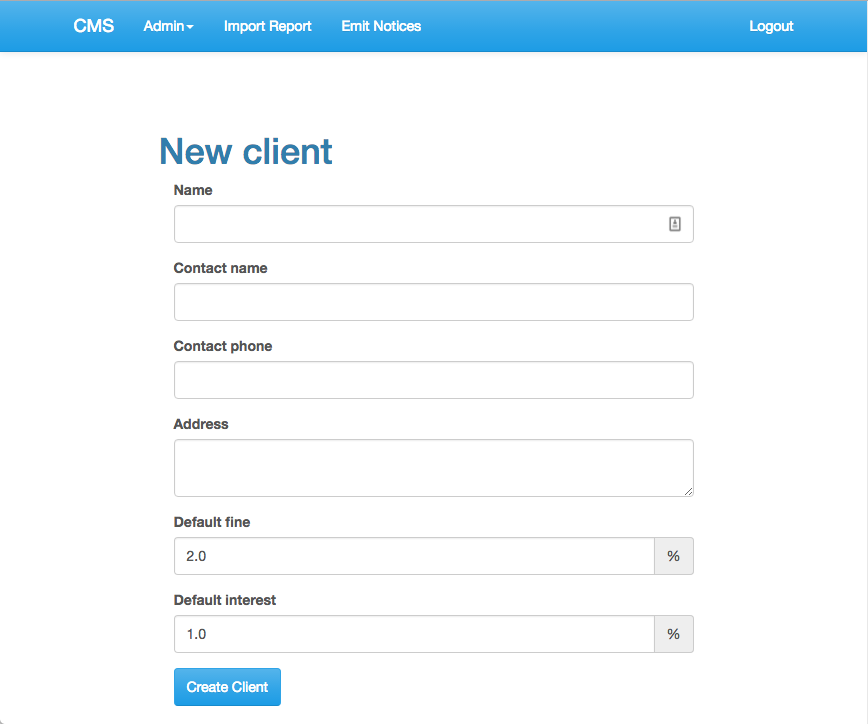
\includegraphics[scale=0.25]{./images/ss/client/create/3.png}
    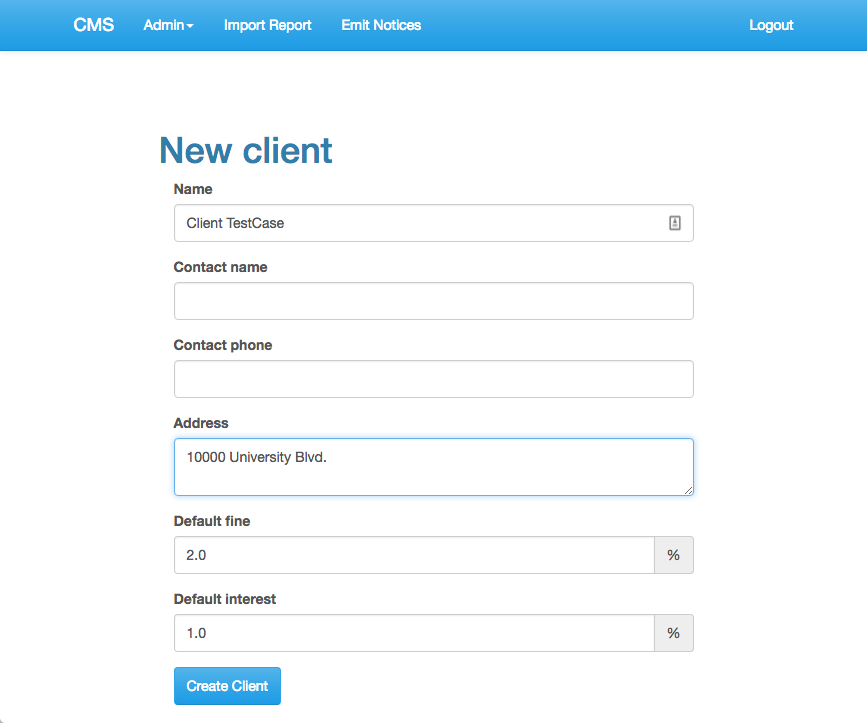
\includegraphics[scale=0.25]{./images/ss/client/create/4.png}\\
    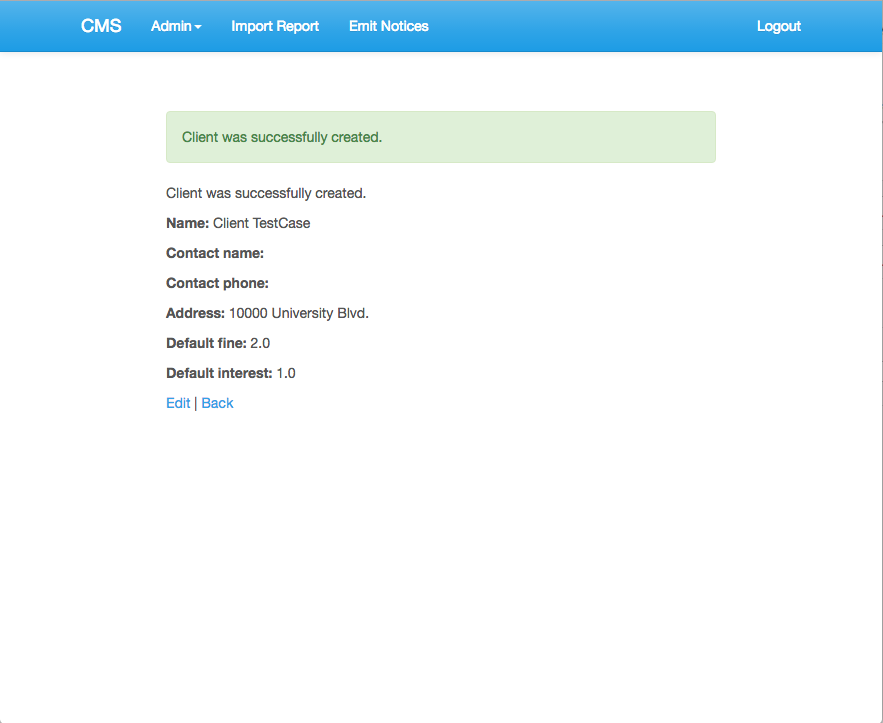
\includegraphics[scale=0.25]{./images/ss/client/create/5.png}
\end{itemize}

\subsection*{Edit a client}

\begin{itemize}
  \item[] \textbf{Trigger:} User interaction with CMS window
  \item[] \textbf{Precondition:} Assert that user is in the Client page and the client to edit is existed
  \item[] \textbf{Path:}
    \begin{enumerate}
      \item User clicks on Edit behind the information of the client who will be edited
      \item User edit new information in the form
      \item User clicks ``Update Client'' button
      \item ``Client successfully updated'' massage is shown
    \end{enumerate}
  \item[] \textbf{Requirements:}
    \begin{enumerate}
      \item The updated client’s new data should be updated to the database
      \item The updated client’s new information should be displayed in the homepage correctly
      \item The clients’ information should be listed in the modification order
    \end{enumerate}
  \item[] \textbf{Screenshots:}\\
    \includegraphics[scale=0.25]{./images/ss/client/edit/1.png}
    \includegraphics[scale=0.25]{./images/ss/client/edit/2.png}\\
    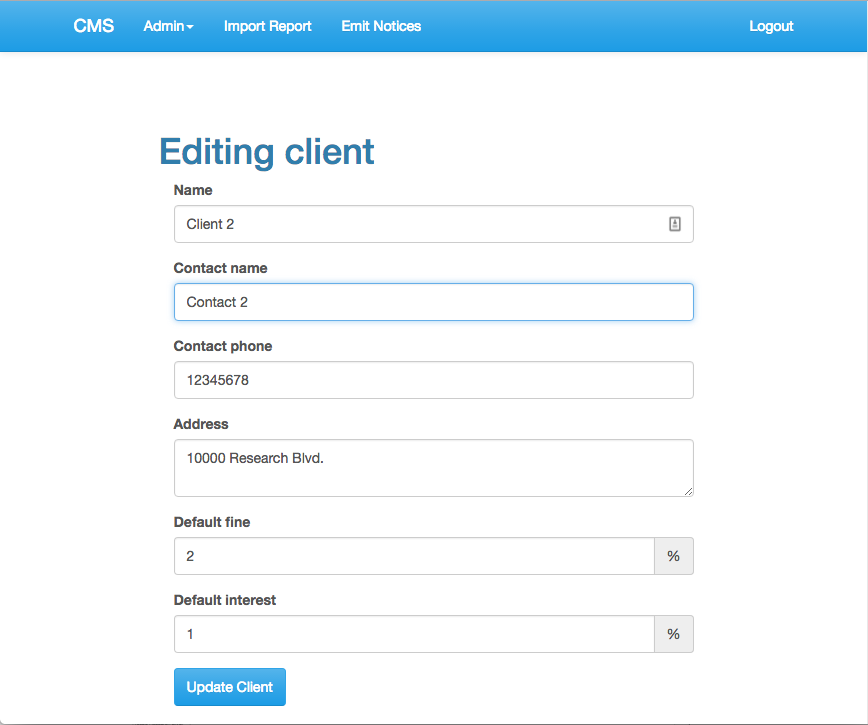
\includegraphics[scale=0.25]{./images/ss/client/edit/3.png}
    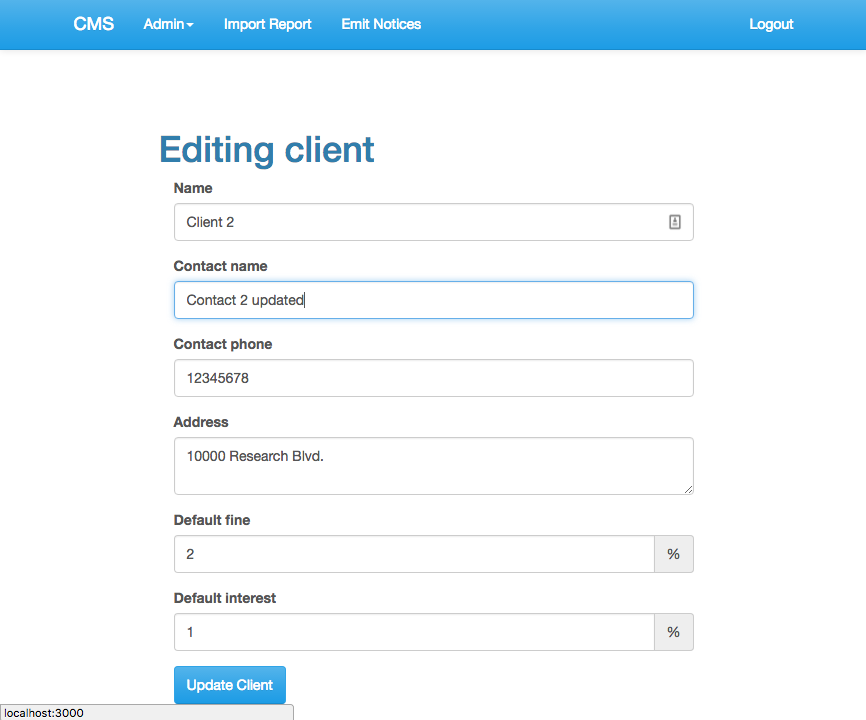
\includegraphics[scale=0.25]{./images/ss/client/edit/4.png}\\
    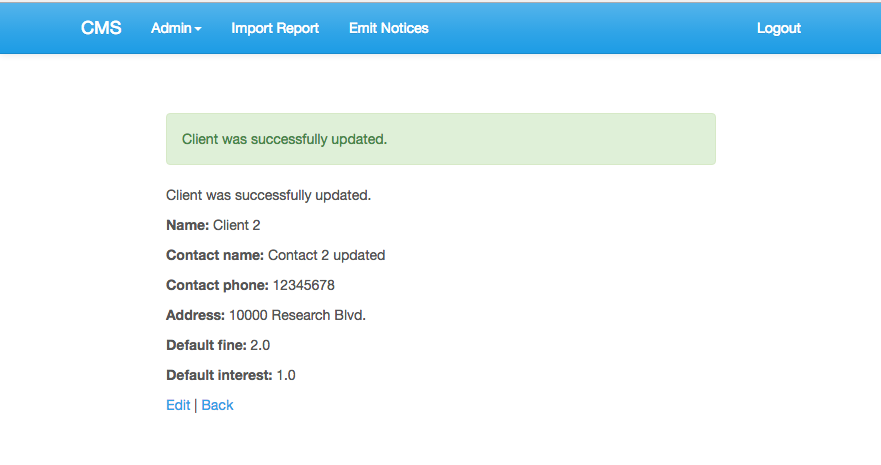
\includegraphics[scale=0.25]{./images/ss/client/edit/5.png}
\end{itemize}

\subsection*{Delete a client}

\begin{itemize}
  \item[] \textbf{Trigger:} User interaction with CMS window
  \item[] \textbf{Precondition:} Assert that user is in the Client page and the client to edit is existed
  \item[] \textbf{Path:}
    \begin{enumerate}
      \item User clicks on Destroy at the end of the information of the client who will be deleted
      \item An alter message says ``Are you sure'' is shown
      \item User clicks ``OK'' button
      \item Client successfully destroyed massage is shown
    \end{enumerate}
  \item[] \textbf{Requirements:}
    \begin{enumerate}
      \item The deleted client’s data should be removed to the database
      \item The deleted client’s information should not be displayed in the homepage
      \item Other clients’ information should be listed as the same as those before deleting
    \end{enumerate}
  \item[] \textbf{Screenshots:}\\
    \includegraphics[scale=0.25]{./images/ss/client/delete/1.png}
    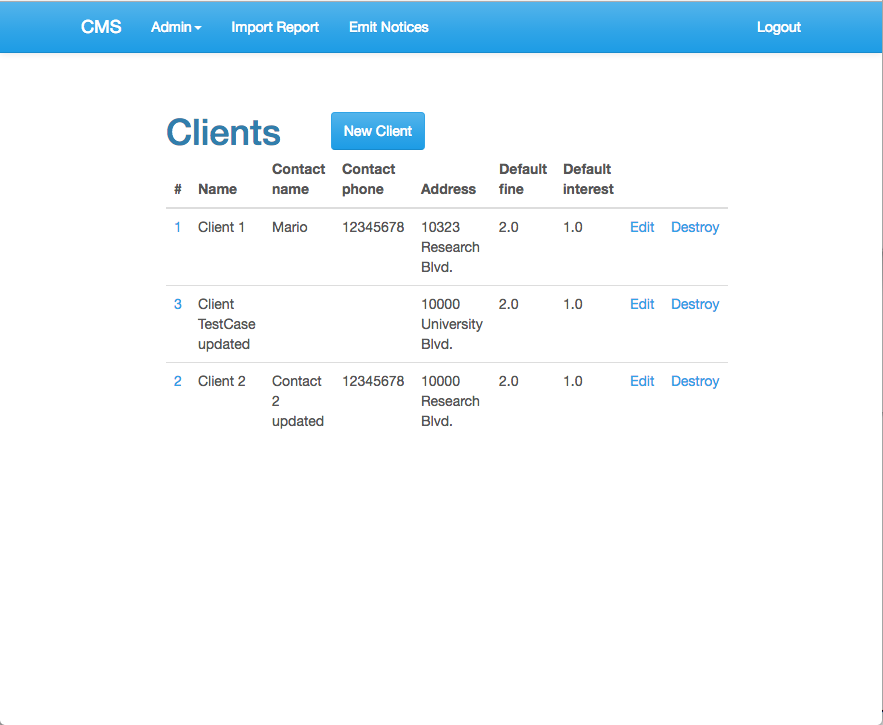
\includegraphics[scale=0.25]{./images/ss/client/delete/2.png}\\
    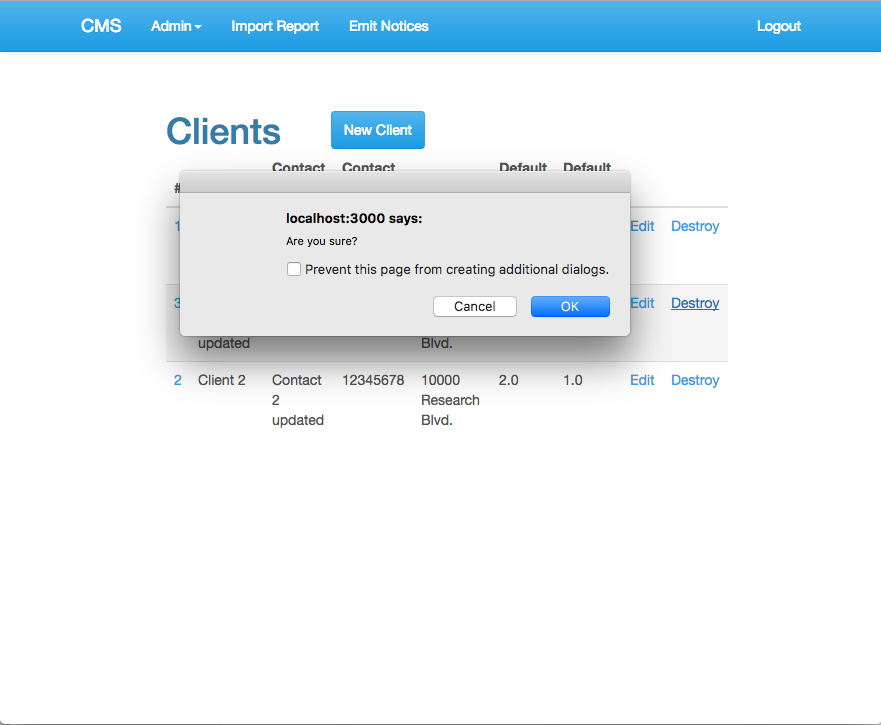
\includegraphics[scale=0.25]{./images/ss/client/delete/3.png}
    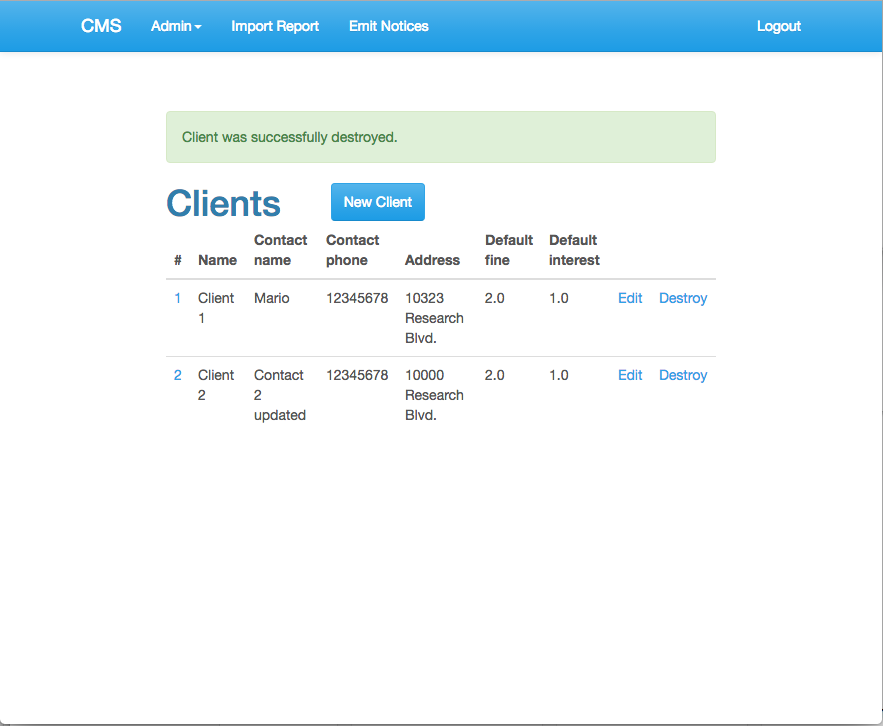
\includegraphics[scale=0.25]{./images/ss/client/delete/4.png}
\end{itemize}
